\documentclass[12pt]{article}
\usepackage[utf8]{inputenc}
\usepackage[T1]{fontenc}
\usepackage{graphicx}
\usepackage{xcolor}
\usepackage{amsmath}

%%novalidate

\usepackage{tikz}
\usepackage{calc}
\usepackage{booktabs}
%\usepackage{hyperref}

% colors
\definecolor{color1}{HTML}{000060}
%\definecolor{color1}{HTML}{8C260F}
\definecolor{color2}{HTML}{333333}


% fonts
\usepackage{fontspec}
\defaultfontfeatures{Mapping=tex-text}
\setmainfont
[BoldFont=Lato-Bold.ttf,
ItalicFont=Lato-Italic.ttf,
BoldItalicFont=Lato-BoldItalic.ttf]
{Lato-Regular.ttf}
\newfontfamily\headingfont[ItalicFont=Lato-BlackItalic.ttf]{Lato-Black.ttf}
%%%

\usepackage{geometry}
\geometry{a4paper,
hmargin=20mm,vmargin=20mm,
head=0ex,foot=3ex}

\linespread{1.3}

\usepackage[hang]{caption}
\DeclareCaptionFormat{upper}{#1#2\uppercase{#3}\par}
\captionsetup{labelfont={bf,color=color2},textfont={normalsize,color=color2},format = upper,figurename=FIGURE,tablename=TABLE}

%%% fancy sections
\usepackage{titlesec}
%\titleformat{\chapter}{\headingfont\LARGE\bfseries\scshape\color{color1}}{\thechapter}{1em}{}[\titlerule]
\titleformat{\section}{\color{color1}\headingfont\Large\bfseries\uppercase}{\thesection}{1em}{}[\titlerule]
\titleformat{\subsection}{\color{color1}\headingfont\large\bfseries\uppercase}{\thesubsection}{1em}{}
\titleformat{\subsubsection}{\color{color1}\headingfont\bfseries\uppercase}{\thesubsubsection}{1em}{}
%%%

% head and foot
\usepackage{fancyhdr}
\pagestyle{fancy}
\lhead{}
\chead{}
\makeatletter
\rhead{\color{color2}\@date}
\makeatother
\newlength{\myheight}
\lfoot{
\settoheight{\myheight}{\thepage}
\raisebox{-2ex-0.5\myheight}{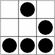
\includegraphics[height=4ex]{logo}}
}
\cfoot{\color{color2} Guide: Prof. Gopal R Patil}
\rfoot{\color{color2}\thepage}
\renewcommand\headrulewidth{0pt}
\renewcommand\footrulewidth{0pt}

%%% picture on cover page
\usepackage{eso-pic}
\newcommand\BackgroundPic{%
\put(0,0){%
\parbox[b][\paperheight]{\paperwidth}{%
\vfill
\centering

\includegraphics[width=\paperwidth,height=\paperheight,%
keepaspectratio]{cover}%
\vfill
}}}
%%%
% custom titlepage
\makeatletter
\renewcommand{\maketitle}{
\thispagestyle{empty}
\AddToShipoutPicture*{\BackgroundPic}
\ClearShipoutPicture
%
\phantom{a}
\vfill
\phantom{a}\hfill
\begin{tabular}[c]{@{}p{0.7\textwidth}@{}}
      \color{white}\headingfont\LARGE\@title\\[1em]
      \color{white}\headingfont\Large\@author\\[2em]
    %   \color{white}\headingfont\Large\@coauthor\\[2em]
\end{tabular}
%
\clearpage
}
\makeatother
%%%


%%% fancy boxes
\usepackage{tcolorbox}
\usepackage{wrapfig}
\def\fullboxbegin{
\bigskip
\begin{tcolorbox}[colback=color1,colframe=color1,coltext=white,arc=0mm,boxrule=0pt]
}
\def\fullboxend{\end{tcolorbox}\medskip}
%
\def\leftboxbegin{
\begin{wrapfigure}{l}{0.5\textwidth}
\begin{tcolorbox}[colback=color1,colframe=color1,coltext=white,arc=0mm,boxrule=0pt]
}
\def\leftboxend{
\end{tcolorbox}
\end{wrapfigure}
}
%
\def\rightboxbegin{
\begin{wrapfigure}{r}{0.5\textwidth}
\begin{tcolorbox}[colback=color1,colframe=color1,coltext=white,arc=0mm,boxrule=0pt]
}
\def\rightboxend{
\end{tcolorbox}
\end{wrapfigure}
}
%
\newcounter{frames}
\def\frameboxbegin#1{
\bigskip
\refstepcounter{frames}
\begin{tcolorbox}[colback=white,colframe=color1,arc=0mm,title={\MakeUppercase{\textbf{Frame \arabic{frames}}: #1}}]
}
\def\frameboxend{
\end{tcolorbox}
}
%%%

\usepackage{lipsum}

%%%%%%%%%%%%%%%
% Title Page

\huge\color{white} \hspace{-6mm}The Use of Entropy Maximization \\Models in the Theory of \\Trip Distribution, Mode Split \\and Route Split 
\vspace{5mm}
\title{Critique on reasearch paper}
\author{\newline Ayush Pandey - 150040087 \newline Amogha Hakkare Arunachala - 150040102 \newline Priyharsh Gangwar - 150040089 \newline Ashwini Kumar Singh - 150040040 }
% \coauthor{Priyharsh Gangwar \newline 150040102 \newline Indian Institute of Technology Bombay}
\date{\today}
%%%%%%%%%%%%%%%


%%%%%%%%%%%%%%%

\begin{document}
\maketitle

% \tableofcontents
\color{black}
% \clearpage

\section{Introduction}

\subsection{About the paper}

\noindent \color{black} \textbf{The Use of Entropy Maximization Models in the Theory of Trip Distribution, Mode Split and Route Split} is the paper, authored by \textbf{\emph{A. G. Wilson}} from University College London. The paper was accepted and published in the \textbf{Journal of Transport Economics and Policy} in \textbf{October 1998}.


\subsection{Context of The Work}
The four-stage Transportation Demand Model is the most widely used model for Transportation Forecasting. The four stages of the model are -- Trip generation, Trip Distribution, Modal Split and Traffic Assignment. The different stages within the model have different models to obtain the trips generated, distribute the generate trips, split the trips mode wise and assign traffic to various links. While the Trip generation model is obtained by conducting extensive surveys, collecting socioeconomic data and performing regression, cross category or various other analysis. The most popular method for Trip Distribution is the \textbf{Gravity Model} which is a modification of the \textbf{Furness Method}. The Mode Split multinomial logit model is based on the utility maximization and the Traffic Assignment models are usually based on cost minimization.

\subsection{Purpose of the Work}

The author does not concerns with the Trip Generation and assumes that the trip ends are already known. The paper tries to use a new method to construct the Distribution and Modal Split models. The author uses the Entropy maximization method to populate the Origin-Destination (OD) or the Production Attraction Matrix (PA) matrix.\\

\newline Our critique focuses on the formulation of the Entropy Maximization problem, various constraints associated with it and the types of solutions obtained based on the constraints considered.
\newpage

\section{Entropy Maximization}


\subsection{Motivation}

Wilson looked at Trip Distribution problem in a totally different way, independent from the models already being used.
\frameboxbegin{Principal of Maximum Entropy}
\textbf{The Principal of Maximum Entropy states that the probability distribution that best represents the current state of knowledge is the one with largest Entropy} 
\frameboxend
Wilson divided the trip distribution into different states, and the decision variables in the Trip Distribution Problem are the number of trips between any given pair of zones ($T_{ij}$). 
\begin{enumerate}
    \item Micro-state $\rightarrow$ Individual Trips
    \item Meso-state $\rightarrow$ Number of trips between pair of zones ($T_{ij}$)
    \item Macro-state $\rightarrow$ Overall matrix with total trips
\end{enumerate}
\vspace{-5mm}
\subsection{Notation}
\begin{enumerate}
    \item C $\rightarrow$ The cost matrix
    \item $c_{ij} \rightarrow$ The cost to travel between zone i and j
    \item $T_{ij} \rightarrow$ The number of trips between zone i and j
    \item $T(C) \rightarrow$ The Trip Distribution Matrix
    \item $W[T(C)] \rightarrow$ The number of ways the individual trips can be distributed to the OD matrix  
    \item T $\rightarrow$ Total number of trips
    \item $O_{i} \rightarrow$ Total origins from zone i
    \item $D_{j} \rightarrow$ Total destinations to zone j
\end{enumerate}

\subsection{Entropy associated with a given State of the OD matrix}
The entropy associated with a given OD matrix is the number of ways the micro-state can be decided given that we know the meso-state. This means, in how many ways can the individual trips be chosen from the complete set of trips.
The number of ways $T_{ij}$ trips can be selected from T trips is $T \choose T_{ij}$.
\newline Now the ways of filling the matrix is the product of all these choices which is given in equation (1) which on expanding the binomials becomes equation (2)\\

    \begin{equation}
        W[T(C)] = {T\choose T_{11}} \times {T-T_{11}\choose T_{12}} \times {T-T_{11}-T_{12}\choose T_{13}} \times {.......} \times {T_{mn} \choose T_{mn}}
    \end{equation}
    \begin{equation}
        W[T(C)] = {\frac{T!}{T_{11}!(T - T_{11})!}} \times {\frac{(T - T_{11})!}{T_{12}!(T - T_{11} - T_{12})!}} \times .......
    \end{equation}
The terms cancel out each other and we are left with equation (3)
    \begin{equation}
        W[T(C)] = \frac{T!}{\prod_{i=1,j=1}^{m,n}T_{ij}!}
    \end{equation}

\subsection{Formulation}
Given that the most probable Trip Distribution matrix is the one with the highest entropy, we need to maximize W[T(C)] subject to certain constraints. The decision variables are the $T_{ij}$'s and the constraints are going to be the origins and destinations to a particular zone.
    \begin{equation*}
    \begin{aligned}
    & \underset{T_{ij}}{\text{max}}
    & & \mathrm{}W[T(C)] \\
    & \text{subject to}
    & &  \sum_{j}T_{ij} = O_{i}\\
    &&& \sum_{i}T_{ij} = D_{j}
    \end{aligned}
    \end{equation*}
    
optimizing this objective function is hard so we take $\ln{W}$ to ease the process
    \begin{equation}
        \ln{W} = \ln{T!} - \sum_{i=1,j=1}^{m,n}\ln{T_{ij}}!
    \end{equation}
using Sterling's approximation we can write this as
    \begin{equation}
        \ln{W} = \ln{T!} - \sum_{i=1,j=1}^{m,n}(T_{ij}\ln{T_{ij}} - T_{ij})
    \end{equation}
given that T is a constant we can now write the same optimization problem as
    \begin{equation*}
    \begin{aligned}
    & \underset{T_{ij}}{\text{max}}
    & & \mathrm{}-\sum_{i=1,j=1}^{m,n}(T_{ij}\ln{T_{ij}} - T_{ij}) \\
    & \text{subject to}
    & &  \sum_{j}T_{ij} = O_{i}\\
    &&& \sum_{i}T_{ij} = D_{j}
    \end{aligned}
    \end{equation*}

\newpage

\subsection{Solution}
The constraints can be augmented in to the objective function using Lagrange Multipliers. The objective function then becomes
    \begin{equation}
        -\sum_{i=1,j=1}^{m,n}(T_{ij}\ln{T_{ij}} - T_{ij}) + \sum_{i}\lambda_{i}(O_{i} - \sum_{j}T_{ij}) + \sum_{j}\lambda_{j}(D_{j} - \sum_{i}T_{ij})
    \end{equation}
For maximizing it, we can take the partial derivative of (6) and equate it to zero
    \begin{equation}
        -\ln{T_{ij}} - \lambda_{i} - \lambda_{j} = 0
    \end{equation}
    \begin{equation}
        \longrightarrow T_{ij} = \exp{(-\lambda_{i}-\lambda_{j})}
    \end{equation}
Substituting this into the constraints we get
    \begin{equation}
        \sum_{j}T_{ij} = O_{i} \longrightarrow \sum_{j}\exp{(-\lambda_{i}-\lambda_{j})} = O_{i}
    \end{equation}
    \begin{equation}
        \exp{(-\lambda_{i})} = \frac{O_{i}}{\sum_{j}exp{(-\lambda_{j})}}
    \end{equation}
Let $\frac{\exp{(-\lambda_{i})}}{{O_{i}}} = A_{i}$ and similarly $\frac{\exp{(-\lambda_{j})}}{{{D_{j}}}} = B_{j}$, then 
    \begin{equation}
        T_{ij} = A_{i}O_{i}B_{j}D_{j}
    \end{equation}


\section{Discussion}
Although we started from a totally different point, the result we get from Entropy Maximization is actually the Furness Method. Similarly adding different constraints can yield different models. Although Furness Method is a popular method, it doesn't really takes the impedance to travel between the zones in account. Other models which take the impedance into account can also be obtained from Entropy maximization by adding other constraints.
Desired models can be obtained by using suitable constraints, this beats the point of using a different approach that explores the problem from a whole new perspective.
\subsection{Gravity Model}
Gravity model is an extension of Furness method where $T_{ij} = A_{i}O_{i}B_{j}D_{j}f(c_{ij})$, $f(c_{ij})$ is the deterrence to travel between zone i and j where $c_{ij}$ is the cost of travel between zone i and j. The gravity is obtained from entropy maximization if we add a constraint that the total cost of the system is constant.
    \begin{equation}
        \sum_{i=1,j=1}^{m,n}T_{ij}c_{ij} = C'
    \end{equation}
The objective function after Lagrangian now becomes
\begin{equation}
        -\sum_{i=1,j=1}^{m,n}(T_{ij}\ln{T_{ij}} - T_{ij}) + \sum_{i}\lambda_{i}(O_{i} - \sum_{j}T_{ij}) + \sum_{j}\lambda_{j}(D_{j} - \sum_{i}T_{ij}) + \beta(C' - \sum_{ij}T_{ij}c_{ij})
    \end{equation}
which on solving becomes
    \begin{equation}
        T_{ij} = \exp{(-\lambda_{i}-\lambda_{j}-\beta c_{ij})}
    \end{equation}
which from equation (11) is
    \begin{equation}
        T_{ij} = A_{i}O_{i}B_{j}D_{j}\exp{(-\beta c_{ij})}
    \end{equation}
This is the gravity model with an exponential deterrence function, similarly we can obtain the power deterrence function and gamma deterrence function by using constraints in (16) and the sum of (15) and (16) respectively
    \begin{equation}
        \sum_{i=1,j=1}^{m,n}T_{ij}\ln{c_{ij}} = C'
    \end{equation}
    
Although the Entropy Maximization model validates the Gravity and Furness method, it should not be treated as concrete proof, to begin with the concept of entropy maximization from statistical mechanics, then we can get the models we want by playing with the constraints and hence many models can be verified using this approach.


% \section{Critical Evaluation}

% \subsection{Introduction of slack variables}
% \vspace{-3mm}

% \frameboxbegin{Defenition}
% Slack variables are used in particular in linear programming. As with the other variables in the augmented constraints, the slack variable cannot take on negative values, as the simplex algorithm requires them to be positive or zero.
% \frameboxend

% Introducing new variables called as the Slack variables is a \textbf{very good idea by the author.} Slack variables are defined appropriately as \textbf{“A mathematical
% representation of
% surplus resources.”} In
% real-life problems, it’s
% unlikely that all
% resources will be used
% completely, so there
% usually are \textbf{unused
% resources.}

% \vspace{-2mm}
% \subsection{Idea of simplex tableau}

\newpage
\section{Conclusions}

 The author has explored a number of questions in depth concerning the \textbf{relation of trip
 distribution to modal split, modal split to route split}, and the form of composite
 impedance functions which relate directly observed costs to "perceived" (or
 "theoretically constructed") costs. A range of empirical tests has been outlined. \\
 \newline
 Modal split models aim to determine the number of trips on different modes given the travel demand between different pairs of nodes (zones). These models try to mathematically describe the mode choice phase of the sequential demand analysis procedure. Generally, choice models are used for modal split analysis.
 \\
 \newline
 \textbf{Trip generation} is the first step in the conventional four-step transportation forecasting process (followed by \textbf{trip distribution, mode choice, and route assignment}), widely used for forecasting travel demands.\\
 \newline The
 results, as well as possibly laying the foundation for better forecasting models,
 would tell us something about the way in which travellers perceive modes,
 routes and costs. One difficulty in carrying out a wide range of tests will be that
 data on route choice is rather difficult to obtain. This is the difficulty or possibly a negative point which everybody faces while implementing a research paper. Obtaining trust-able data from a reliable source is one of the major challenges. \\
 
 There remain, of course, a number
 of tests to carry out on the mechanism of distribution models themselves, especially
 the generalized model represented by the above mentioned equations and its various aggregates

\end{document}          
